\section{True Heading Signal}
% ➢ A5.2 Determine a True Heading Signal to test your system – this is the bearing the aircraft is travelling on at any moment in time. To illustrate the behaviour of the system best, consider a small or medium sized UAV – Simulate a few minutes of flight that might include typical features: straight flight, high and low rate turns, buffeting from gusts etc. (Tip: try and ensure you can see the non-ideal response of both of the individual sensors when their outputs are plotted on a graph. Depending on your heading signal, your system may be well behaved and not demonstrate all sensor behaviour. If this is the case introduce more extreme features in the heading signals). (10 marks)

The heading signal aims to comprehensively test the response of the sensor system for a range of real frequencies. The heading changes modelled were realistically tuned for a small UAV, such as a DJI Mavic 2 \cite{mavic2} with a turning rate capability of 200 $\degree/s$ since it helps characterize the sensor system combination. For slower UAVs, the sensor system response limitations do not change, although the heading signal differentials would be slower. Dorobantu et al. \cite{dorobantu2011frequency} identify a number of flight dynamic frequencies of small, low cost fixed-wing UAVs that are considered in this model. The applicable frequency range that describes the majority of their relevant aircraft dynamics is suggested to be between $10^{-1}$ and $10^1$ $rad/s$ for their aircraft, although potentially faster UAVs prone to influence by higher frequencies. For reference, spiral, dutch roll, and rolling flight lateral/directional movements within the yaw angle X-Y plane introduce frequencies of 0.021, 6.102 and 14.912 $rad/s$ respectively. The DJI Mavic 2 flys differently and experiences other forces not considered by this model, and this is why the heading signal should mainly excite directional movements within these frequencies. Figure \ref{fig:raw_heading_signal} describes the selected heading signal. 

\begin{figure}[h]
    \centering
    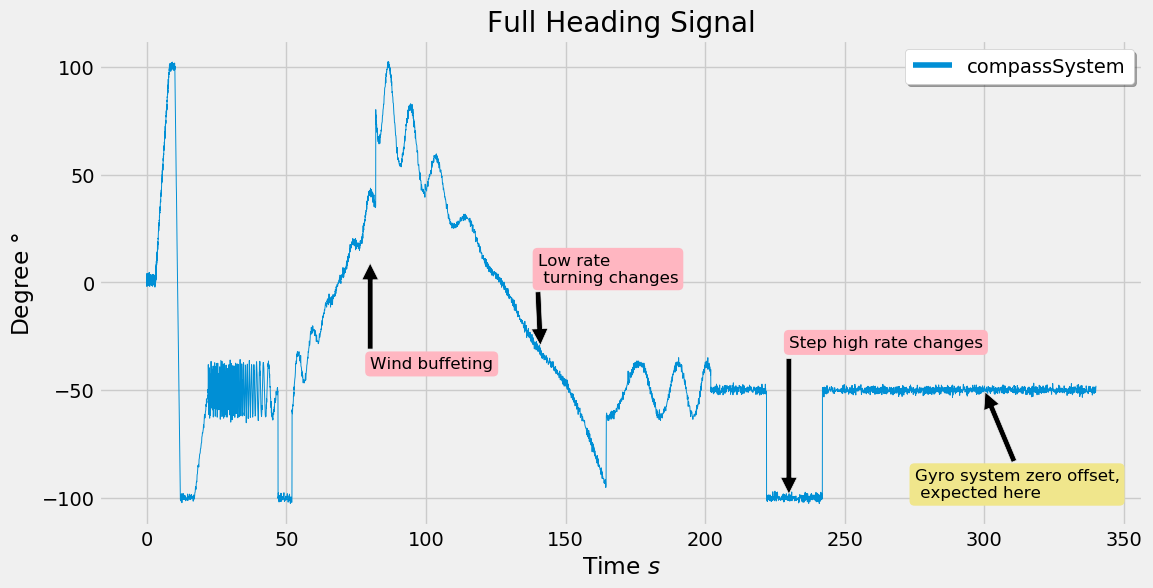
\includegraphics[width=\linewidth]{img/fullHeadingSignal.png}
    \caption{Complete heading signal.}
    \label{fig:raw_heading_signal}
\end{figure}

\begin{figure}[h]
    \centering
    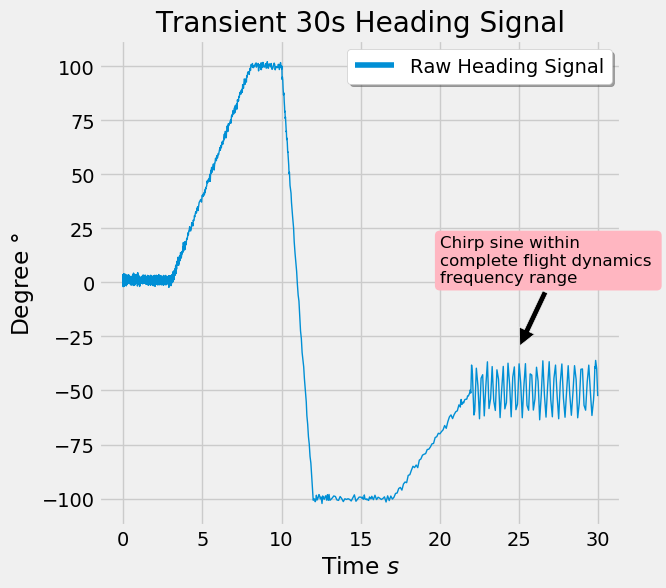
\includegraphics[width=0.75\linewidth]{img/headingSignal30s.png}
    \caption{Initial 30s of the heading signal.}
    \label{fig:transient_heading_signal}
\end{figure}

The heading signal can be separated into two analysis sections. From seconds 0 to 70, higher frequency changes aim to describe the transient response at the very limit of the DJI Mavic 2 physical operation. Part of this region is illustrated in Figure \ref{fig:transient_heading_signal}, although zoomed in to provide more detail. Drastic changes from 100 to -100 degrees are observed in a space of 3 seconds at the start, close to the rated turning rate of the DJI Mavic of 200 $\frac{\degree}{s}$. Random noise jitter with a mean of 0.05 $\degree$ has been added to the complete heading siganl to the minor imperfections in directional flight as can be individually noticed within the step signal or straight flight towards the end. The chirp sinusoidal wave between seconds 22 to 47 decreases frequency from 20 Hz to 0.01 Hz, within the range of most flight dynamics vibrations suggested by \cite{dorobantu2011frequency}. Mainly steep change slopes are observed at seconds 10, 20, 47 and 52 aim to demonstrate high rate turns.

The second section aims to test slower changes from second 70 onwards. Low rate turns with wind buffeting is described between seconds 50 to 120. Between seconds 160 and 210, sinusoidal waves also aim to demonstrate further low frequency behaviour. The rate gyro zero offset is expected to be observed towards the straight end of the heading flight.

During the design of the heading signal, several standard input signals such as the saw-tooth, sine, step, and delta waves with varying frequencies were independently inputted to understand the specific response of the system and design the heading signal for several frequency behaviours. Most of these independent signal responses are displayed within this heading signal.

